\documentclass{article} \usepackage{tabularx}
\usepackage{amsmath} \usepackage{amssymb} \usepackage{tikz}
\usetikzlibrary{timeline} \usepackage{booktabs}
\usepackage{float} \restylefloat{table} \graphicspath{{images/}}
\usepackage[margin={3.5cm,3cm}]{geometry} \usepackage{multicol}
\setlength\columnsep{1.5cm} \usepackage{tabto}
\usepackage{pdflscape} \usepackage{graphicx} \usepackage{array}
\usepackage[T1]{fontenc} \usepackage[utf8]{inputenc}
\usepackage{charter} \usepackage{environ} \usepackage{tikz}
\usetikzlibrary{calc,matrix}
% For citations
\usepackage[sort,numbers]{StyFiles/natbib}
\renewcommand{\citename}{\citet} \renewcommand{\cite}{\citep}
\usepackage{StyFiles/natbibspacing}


% code by Andrew: http://tex.stackexchange.com/a/28452/13304
\makeatletter \let\matamp=& \catcode`\&=13 \makeatletter
\def&{\iftikz@is@matrix \pgfmatrixnextcell \else \matamp \fi}
\makeatother

\newcounter{lines} \def\endlr{\stepcounter{lines}\\}

\newcounter{vtml} \setcounter{vtml}{0}

\newif\ifvtimelinetitle \newif\ifvtimebottomline
\tikzset{description/.style={ column 2/.append style={#1} },
  timeline color/.store in=\vtmlcolor, timeline
  color=red!80!black, timeline color
  st/.style={fill=\vtmlcolor,draw=\vtmlcolor}, use timeline
  header/.is if=vtimelinetitle, use timeline header=false, add
  bottom line/.is if=vtimebottomline, add bottom line=false,
  timeline title/.store in=\vtimelinetitle, timeline title={},
  line offset/.store in=\lineoffset, line offset=4pt, }

\NewEnviron{vtimeline}[1][]{%
  \setcounter{lines}{1}%
  \stepcounter{vtml}%
  \begin{tikzpicture}[column 1/.style={anchor=east}, column
    2/.style={anchor=west}, text depth=0pt,text height=1ex, row
    sep=1ex, column sep=1em, #1 ]
    \matrix(vtimeline\thevtml)[matrix of nodes]{\BODY};
    \pgfmathtruncatemacro\endmtx{\thelines-1} \path[timeline
    color st] ($(vtimeline\thevtml-1-1.north
    east)!0.5!(vtimeline\thevtml-1-2.north west)$)--
    ($(vtimeline\thevtml-\endmtx-1.south
    east)!0.5!(vtimeline\thevtml-\endmtx-2.south west)$);
    \foreach \x in {1,...,\endmtx}{ \node[circle,timeline color
      st, inner sep=0.15pt, draw=white, thick]
      (vtimeline\thevtml-c-\x) at
      ($(vtimeline\thevtml-\x-1.east)!0.5!(vtimeline\thevtml-\x-2.west)$){};
      \draw[timeline color
      st](vtimeline\thevtml-c-\x.west)--++(-3pt,0); }
    \ifvtimelinetitle%
    \draw[timeline color
    st]([yshift=\lineoffset]vtimeline\thevtml.north west)--
    ([yshift=\lineoffset]vtimeline\thevtml.north east);
    \node[anchor=west,yshift=16pt,font=\large] at
    (vtimeline\thevtml-1-1.north west) {\textsc{Timeline
        \thevtml}: \textit{\vtimelinetitle}}; \else%
    \relax%
    \fi%
    \ifvtimebottomline%
    \draw[timeline color
    st]([yshift=-\lineoffset]vtimeline\thevtml.south west)--
    ([yshift=-\lineoffset]vtimeline\thevtml.south east); \else%
    \relax%
    \fi%
  \end{tikzpicture}
}

\begin{document}


\begin{titlepage}
	\centering
	\begin{figure}[H]
    \centering
    % \includegraphics[scale=0.5]{logo_nasa_trio_black@2x.png}
	\end{figure}
	\vspace{2cm} {\scshape\LARGE Ph.D. Research Proposal\par}
  \vspace{2cm}
  
  %%%%%%%%%%% Title
	{\scshape\LARGE

    Sequence Learning Using Deep Neural Networks With Flexibility
    \& Interpretability
    
    \par} {\huge\bfseries \par}
	
	\vspace{2cm} {\Large\itshape Chang Li\par} \vfill

  {\Large\itshape Supervisor\par} {\Large\itshape Prof. Dacheng
    \textsc{Tao}\par} \vfill

\end{titlepage}


\section{Aims \& Objectives}

\begin{enumerate}
\item Flexibility in modeling complex patterns with long-range
  dependencies
  \begin{enumerate}
  % DA-RNN
  \item Capturing complex non-linear correlations without prior
    knowledge and assumptions
  \item Encoding high dimensional input variables adaptively
  \item Discovering long term dependencies of encoded inputs
  % Capsule
  \item Novel insights in feature extraction of complex inputs
  % \item Demonstrating both classification and regression problems
  \end{enumerate}
\item Network architectures with better computational properties
\item Encoding/Decoding human intepretable representation
  into/from models
  \begin{enumerate}
  \item Learning deep neural networks coupled with structured
    (potentially predefined) latent variable sequence
  \item Approximating deep neural networks' input-output
    relationships using human intepretable models
  \end{enumerate}
\end{enumerate}

\section{Synopsis}
\label{sec:synop}


\section{Background And Literature Review}
\label{sec:intro}

One interesting task in machine learning is modeling complex
sequences having long-term dependencies. Many applications such
as machine translation, complex dynamical system analysis,
activity recognition and behavioral phenotyping tools for
neuro-science involved with capturing non-linear patterns in
sequences. Sequence learning mainly have three difficulties:
approximating non-linear relationship among sequences, feature
selection and capturing long-term dependencies. Our primary aim
of this proposal is mainly focused on demonstrating those three
difficulties. 

Despite substantial effort has been made for modeling sequences,
many of those models are neither unable to approximate non-linear
relationships nor have rigid assumptions due to the dependency on
predefined form of prior function. For example, autoregressive
moving average (ARMA) model~\cite{hibon1997arma} and many of its
variants~\cite{brockwell2013time} have raised interests because
of their effectiveness in many real world applications. However,
those models cannot capturing non-linear relationships.
Probabilistic Graphical
Models~\cite{murphy2012machine,koller2009probabilistic} (PGM) are
very well studied for the past decades. With predefined prior
distributions from domain knowledge, PGMs are capable to encode
many sequence relationships such as Gaussian
Processes~\cite{frigola2014variational}, Hidden Markov
Models~\cite{eddy1996hidden} (HMM) and Linear Dynamic
Systems~\cite{bar1993estimation} (LDS). However, capabilities of
approximating non-linear patterns of PGMs are also severely
suffered from rigid assumptions over priors.

Deep Neural Networks~\cite{goodfellow2016deep} (DNNs) are powerful and flexible models that
have overwhelming performance on various difficult learning tasks
such as image classification, visual object recognition, machine
translation and speech recognition. It can take high dimensional
data with rich structure as input and scales over large data-set.
DNNs are usually composed of hierarchical layers which contains
large amount of latent variables. Non-linearity in the data is
usually captured by non-linear interactions through those latent
variables. Each of these latent variables normally connected to
many other variables in adjacent layers. Results of those unique
distributed representations are that DNNs are extremely flexible
in fixing difficult problems in high dimensional space and have
very generic learning algorithm (Stochastic Gradient Descent,
SGD) for various problems. With sufficient training data, DNNs
usually can get nice approximation of that information in a
reasonable amount of time~\cite{goodfellow2016deep}.

Despite the powerful capability of approximation, one significant
limitation of DNNs is that they require fixed dimension of inputs
and targets. Thus DNNs cannot be applied directly on areas
without prior knowledge about variables' length or have various
input length, such as speech recognition and machine translation.
\citename{sutskever2014sequence} in 2014 demonstrated this
difficulty as sequence to sequence problems. They introduced an
encoder-decoder framework based on two Recurrent Neural Networks
(RNNs) and achieved a very successful result in machine
translation. The key ideas (as shown in Figure~\ref{fig:en-de})
behind encoder-decoder networks and its variants are that they
first encode the whole sentence of words into a single, fixed
length variable using encoder network. Then a decoder network is
used to decode that variable and generate translation. They
enabled the network to take various length of inputs by encoding
each of them into a single and fixed length variable. One major
drawback is that ``indeed the performance of a basic
encoder–decoder deteriorates rapidly as the length of an input
sentence increases~\cite{attention}''. Since for many sequence
learning applications there exists many long-term dependencies
relationships, the question of solving this drawback remains
open.

\begin{figure}
  \centering
  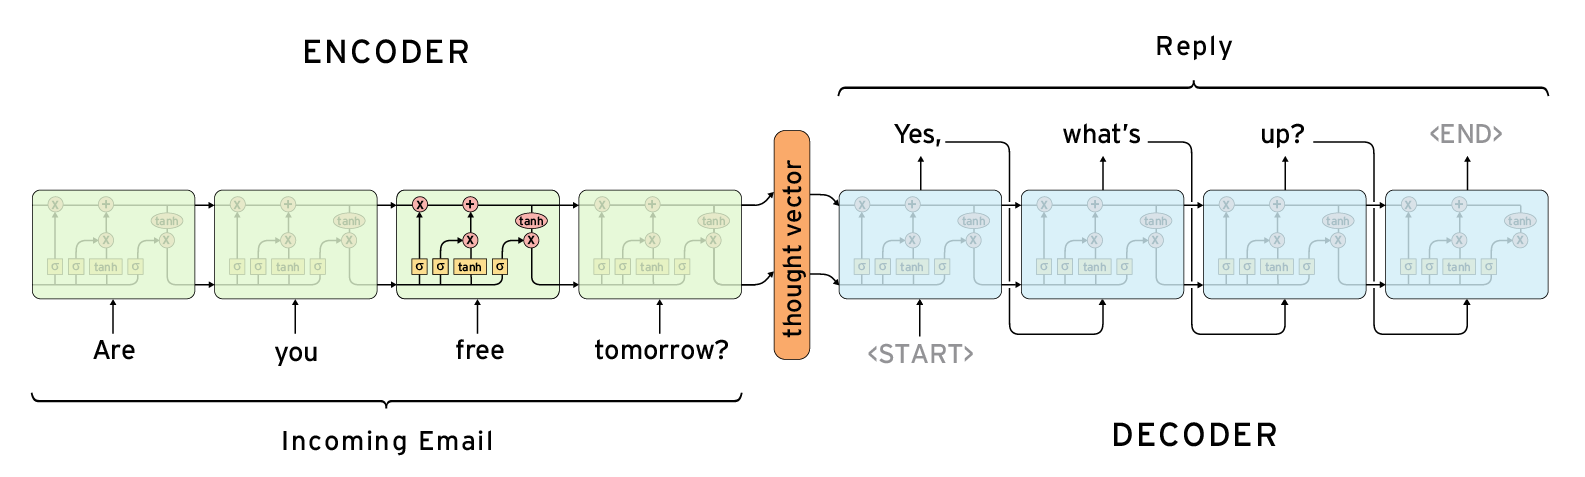
\includegraphics[scale=0.5]{images/en-de.png}
  \caption{Encoder-Decoder Network}
  \label{fig:en-de}
\end{figure}

Other than long-term dependencies difficulty, DNNs'

\section{Expected Research Contribution}
\label{sec:contrib}


\section{Proposed Methodology}
\label{sec:method}


\section{Work Plan}


\bibliographystyle{abbrvnat} \bibliography{proposal.bib}
\end{document}
